% Template for solutions write-ups, STAT 460/560
% Some basic notation is defined in 'macros/basic-math-macros'

\documentclass{article}
\usepackage{verbatim}
\usepackage{titlesec}

\def\coursename{STAT 447C: Bayesian Statistics}
\def\semester{Fall 2024}

\setlength{\oddsidemargin}{0.0 in}
\setlength{\evensidemargin}{0.0 in} 
\setlength{\topmargin}{-0.6 in} 
\setlength{\textwidth}{6.5 in} 
\setlength{\textheight}{8.5 in}
\setlength{\headsep}{0.75 in} 
\setlength{\parindent}{0 in}
\setlength{\parskip}{0.1 in}

\titleformat*{\section}{\Large\bfseries}


% prints box at top of first page with relevant info
\newcommand{\problemset}[3]{
   \pagestyle{myheadings}
   \thispagestyle{plain}
   \newpage
   \noindent
   \begin{center}
   \framebox{
      \vbox{\vspace{2mm}
    \hbox to 6.28in { {\bf \coursename
                        \hfill \semester} }
       \vspace{4mm}
       \hbox to 6.28in { {\Large \hfill #3  \hfill} }
       \vspace{2mm}
       \hbox to 6.28in { {\it #1 \hfill \texttt{#2}} }
      \vspace{2mm}}
   }
   \end{center}
   \vspace*{4mm}
}

\newcommand{\qsol}[1]{\section{#1}}
  % DO NOT CHANGE
% \usepackage{graphicx,amssymb,amsmath,amsthm,mathrsfs}
% \usepackage{multirow,makeidx,algorithmic,algorithm}
\usepackage{multirow,makeidx,algpseudocode,algorithm}
\usepackage{mathtools}
\usepackage{enumitem}
 
\usepackage{parskip}
\usepackage{setspace}
\usepackage{float, graphicx}
\usepackage{adjustbox}
\usepackage{bbm}
\usepackage{tabularx}
\usepackage{subfigure}
\usepackage{amsmath,amssymb,amsfonts,amsthm,amsbsy,amstext,mathrsfs}
\usepackage{hyperref}
\usepackage{url}
\usepackage{color}
\usepackage{graphicx} % Required for inserting images
\usepackage[utf8]{inputenc}

%% reference
\usepackage[round]{natbib}
\bibliographystyle{abbrvnat}
% \usepackage{cite}
% \bibliographystyle{plainurl}
% \bibliographystyle{abbrv}
% \bibliographystyle{plain}
% \bibliographystyle{unsrt}


%% code in-text
\usepackage{listings}
\usepackage{xcolor}

\definecolor{codegreen}{rgb}{0,0.6,0}
\definecolor{codegray}{rgb}{0.5,0.5,0.5}
\definecolor{codepurple}{rgb}{0.58,0,0.82}
\definecolor{backcolour}{rgb}{0.95,0.95,0.92}

\lstdefinestyle{mystyle}{
    backgroundcolor=\color{backcolour},   
    commentstyle=\color{codegreen},
    keywordstyle=\color{magenta},
    numberstyle=\tiny\color{codegray},
    stringstyle=\color{codepurple},
    basicstyle=\ttfamily\footnotesize,
    breakatwhitespace=false,         
    breaklines=true,                 
    captionpos=b,                    
    keepspaces=true,                 
    numbers=left,                    
    numbersep=5pt,                  
    showspaces=false,                
    showstringspaces=false,
    showtabs=false,                  
    tabsize=2
}

\lstset{style=mystyle}


%% layout
\oddsidemargin 3mm
\evensidemargin 3mm
\topmargin -12mm
\textheight 660pt
\textwidth 450pt  % DO NOT CHANGE
% ADD YOUR CUSTOM NOTATION HERE
\newcommand{\R}{\mathbb R}
\newcommand{\Z}{\mathbb Z}
\newcommand{\Q}{\mathbb Q}
\newcommand{\N}{\mathbb N}
\newcommand{\C}{\mathbb{C}}
\newcommand{\1}{\mathbbm{1}}
\newcommand{\E}{\mathbb E}
\newcommand{\Mcal}{{\cal M}}
\newcommand{\Ncal}{{\cal N}}
\newcommand{\Acal}{{\cal A}}
\newcommand{\Bcal}{{\cal B}}
\newcommand{\Fcal}{{\cal F}}
\newcommand{\Ecal}{{\cal E}}
\newcommand{\Gcal}{{\cal G}}
\newcommand{\Hcal}{{\cal H}}
\newcommand{\Scal}{{\cal S}}
\newcommand{\Xcal}{{\cal X}}
\newcommand{\Lcal}{{\cal L}}
\newcommand{\Mscr}{\mathscr{M}}
\newcommand{\eps}{\varepsilon}
\renewcommand{\P}{\mathbb P}
\DeclareMathOperator{\Var}{Var}
\DeclareMathOperator{\Poi}{Poi}
\DeclareMathOperator{\Cov}{Cov}
\DeclareMathOperator{\Exp}{Exp}
\DeclareMathOperator{\Bin}{Bin}
\DeclareMathOperator{\Geom}{Geom}
\DeclareMathOperator{\Unif}{Unif}
\DeclareMathOperator{\Bernoulli}{Bernoulli}
\DeclareMathOperator{\BetaMP}{BetaMP}
\DeclareMathOperator{\Beta}{Beta}
\newcommand{\abs}[1]{\left|#1\right|}
\newcommand{\norm}[1]{\left\lVert#1\right\rVert}
\newcommand{\floor}[1]{\lfloor#1\rfloor}
\newcommand{\ceil}[1]{\lceil#1\rceil}
\newcommand{\ds}{\displaystyle}
\newcommand{\inv}[1]{#1^{-1}}
\newcommand{\vect}[1]{\boldsymbol{#1}}
\DeclareMathOperator*{\argmax}{arg\,max}
\DeclareMathOperator*{\argmin}{arg\,min}
\newcommand{\convdist}[0]{\overset{d}{\longrightarrow}}
\newcommand{\convprob}[0]{\overset{p}{\longrightarrow}}
\newcommand{\convas}[0]{\overset{a.s.}{\longrightarrow}}
\newcommand{\partiald}[1]{\frac{\partial}{\partial{#1}}}
\newcommand{\partialdd}[1]{\frac{\partial^2}{\partial{#1^2}}}
% \newtheorem{definition}{Definition}[section]
% \newtheorem{theorem}{Theorem}[section]
% \newtheorem{corollary}{Corollary}[theorem]
% \newtheorem{lemma}{Lemma}[theorem]
% \newtheorem{proposition}[theorem]{Proposition}

\newtheorem{definition}{Definition}[section]
\newtheorem{theorem}{Theorem}[section]
\newtheorem{corollary}{Corollary}[section]
\newtheorem{lemma}{Lemma}[section]
\newtheorem{proposition}{Proposition}[section]
\newtheorem*{remark}{Remark}

\renewcommand{\algorithmicrequire}{ \textbf{Input:}} %Use Input in the format of Algorithm
\renewcommand{\algorithmicensure}{ \textbf{Output:}} %UseOutput in the format of Algorithm


%%
% full alphabets of different styles
%%

% bf series
\def\bfA{\mathbf{A}}
\def\bfB{\mathbf{B}}
\def\bfC{\mathbf{C}}
\def\bfD{\mathbf{D}}
\def\bfE{\mathbf{E}}
\def\bfF{\mathbf{F}}
\def\bfG{\mathbf{G}}
\def\bfH{\mathbf{H}}
\def\bfI{\mathbf{I}}
\def\bfJ{\mathbf{J}}
\def\bfK{\mathbf{K}}
\def\bfL{\mathbf{L}}
\def\bfM{\mathbf{M}}
\def\bfN{\mathbf{N}}
\def\bfO{\mathbf{O}}
\def\bfP{\mathbf{P}}
\def\bfQ{\mathbf{Q}}
\def\bfR{\mathbf{R}}
\def\bfS{\mathbf{S}}
\def\bfT{\mathbf{T}}
\def\bfU{\mathbf{U}}
\def\bfV{\mathbf{V}}
\def\bfW{\mathbf{W}}
\def\bfX{\mathbf{X}}
\def\bfY{\mathbf{Y}}
\def\bfZ{\mathbf{Z}}

% bb series
\def\bbA{\mathbb{A}}
\def\bbB{\mathbb{B}}
\def\bbC{\mathbb{C}}
\def\bbD{\mathbb{D}}
\def\bbE{\mathbb{E}}
\def\bbF{\mathbb{F}}
\def\bbG{\mathbb{G}}
\def\bbH{\mathbb{H}}
\def\bbI{\mathbb{I}}
\def\bbJ{\mathbb{J}}
\def\bbK{\mathbb{K}}
\def\bbL{\mathbb{L}}
\def\bbM{\mathbb{M}}
\def\bbN{\mathbb{N}}
\def\bbO{\mathbb{O}}
\def\bbP{\mathbb{P}}
\def\bbQ{\mathbb{Q}}
\def\bbR{\mathbb{R}}
\def\bbS{\mathbb{S}}
\def\bbT{\mathbb{T}}
\def\bbU{\mathbb{U}}
\def\bbV{\mathbb{V}}
\def\bbW{\mathbb{W}}
\def\bbX{\mathbb{X}}
\def\bbY{\mathbb{Y}}
\def\bbZ{\mathbb{Z}}

% cal series
\def\calA{\mathcal{A}}
\def\calB{\mathcal{B}}
\def\calC{\mathcal{C}}
\def\calD{\mathcal{D}}
\def\calE{\mathcal{E}}
\def\calF{\mathcal{F}}
\def\calG{\mathcal{G}}
\def\calH{\mathcal{H}}
\def\calI{\mathcal{I}}
\def\calJ{\mathcal{J}}
\def\calK{\mathcal{K}}
\def\calL{\mathcal{L}}
\def\calM{\mathcal{M}}
\def\calN{\mathcal{N}}
\def\calO{\mathcal{O}}
\def\calP{\mathcal{P}}
\def\calQ{\mathcal{Q}}
\def\calR{\mathcal{R}}
\def\calS{\mathcal{S}}
\def\calT{\mathcal{T}}
\def\calU{\mathcal{U}}
\def\calV{\mathcal{V}}
\def\calW{\mathcal{W}}
\def\calX{\mathcal{X}}
\def\calY{\mathcal{Y}}
\def\calZ{\mathcal{Z}}


%%%%%%%%%%%%%%%%%%%%%%%%%%%%%%%%%%%%%%%%%%%%%%%%%%%%%%%%%%
% text short-cuts
\def\iid{i.i.d.\ } %i.i.d.
\def\ie{i.e.\ }
\def\eg{e.g.\ }
\def\Polya{P\'{o}lya\ }
%%%%%%%%%%%%%%%%%%%%%%%%%%%%%%%%%%%%%%%%%%%%%%%%%%%%%%%%%%

% set theory/measure theory
\def\collection{\calC}
\newcommand{\sigalg}[1]{\mathcal{#1}}
\def\borel{\calB} %Borel sets
\def\sigAlg{\sigalg{H}} %sigma-algebra
\def\filtration{\calF} %filtration
\newcommand{\msblSpace}[1]{(#1,\sigalg{#1})}
\newcommand{\measSpace}[2][\mu]{(#2,\sigalg{#2},#1)}
\newcommand{\borelSpace}[1]{(#1,\borel(#1))}
\newcommand{\measFuncs}[1]{\sigalg{#1}^f}
\newcommand{\pbblSpace}{(\Omega,\sigAlg)}
\newcommand{\probSpace}[1][\bbP]{(\Omega,\sigAlg,#1)}

\def\leb{\lambda}

\def\finv{f^{-1}} % inverse
\def\ginv{g^{-1}} % inverse

% group theory
\def\grp{\calG} %group

% operators
\def\P{\bbP} %fundamental probability
\def\E{\bbE} %expectation
% conditional expectation
\DeclarePairedDelimiterX\bigCond[2]{[}{]}{#1 \;\delimsize\vert\; #2}
\newcommand{\conditional}[3][]{\bbE_{#1}\bigCond*{#2}{#3}}
\def\Law{\mathcal{L}} %law; this is by convention in the literature
% \def\indicator{\mathds{1}} % indicator function
\def\1{{\mathbf 1}}
\def\indicator{\1}

% binary relations
\def\condind{{\perp\!\!\!\perp}} %independence/conditional independence
\def\equdist{\stackrel{\text{\rm\tiny d}}{=}} %equal in distribution
\def\equas{\stackrel{\text{\rm\tiny a.s.}}{=}} %euqal amost surely
\def\simiid{\sim_{\mbox{\tiny iid}}} %sampled i.i.d

% common vectors and matrices
\def\onevec{\mathbf{1}}
\def\iden{\mathbf{I}} % identity matrix
\def\supp{\text{\rm supp}}

% misc
% floor and ceiling
% \DeclarePairedDelimiter{\ceilpair}{\lceil}{\rceil}
% \DeclarePairedDelimiter{\floor}{\lfloor}{\rfloor}
\newcommand{\argdot}{{\,\vcenter{\hbox{\tiny$\bullet$}}\,}} %generic argument dot
%%%%%%%%%%%%%%%%%%%%%%%%%%%%%%%%%%%%%%%%%%%%%%%%%%%%%%%%%%


 
\graphicspath{{./figures/}}







\begin{document}



% FILL IN:
%  - YOUR NAME, YOUR EMAIL (self-explanatory)
%  - The assignment number goes in ##
\problemset{Junsong Tang}{junsong.tang@stat.ubc.ca}{Exercise 7}



% WRITE YOUR SOLUTION TO THE FIRST QUESTION
\qsol{Installing and running Stan} % USE THE SAME TITLES AS ON THE ASSIGNMENT SHEET
\begin{lstlisting}[language=R]
  # 1
  #       mean se_mean   sd  2.5%   25%   50%   75% 97.5% n_eff Rhat
  # p     0.81    0.01 0.16  0.40  0.73  0.85  0.93  0.99   765    1
  # lp__ -3.07    0.03 0.76 -5.39 -3.28 -2.77 -2.56 -2.50   606    1
\end{lstlisting}


\qsol{Regression/classification in Stan}
First, the Stan model is defined as:
\begin{lstlisting}[language=R]
data {
  int<lower=0> N;
  vector<lower=0>[N] t;
  vector<lower=0>[N] y;

}
parameters {
  real<lower=0, upper=200> theta_1;
  real<lower=0, upper=10> theta_2;
  real<lower=0, upper=2*pi()> theta_3;
}
model {
  // prior
  theta_1 ~ uniform(0, 200);
  theta_2 ~ uniform(0, 10);
  theta_3 ~ uniform(0, 2*pi());

  // likelihood
  y ~ poisson(theta1 * (sin(theta2*t + theta3) + 1.1));;
}
\end{lstlisting}

then we run Stan for $2500$ iterations:
\begin{lstlisting}[language=R]
  suppressPackageStartupMessages(require(ggplot2))
  suppressPackageStartupMessages(require(dplyr))

  df = read.csv(
  "https://raw.githubusercontent.com/UBC-Stat-ML/web447/1e345149a5b698ccdf0a7e9b0aeabec2463c50ca/data/sunspots-SN_m_tot_V2.0.csv",
  sep = ";", header=FALSE) %>%
  mutate(count = ceiling(V4)) %>%
  rename(year = V3) %>%
  filter(year > 2005)

  counts = df$count 
  time = df$year

  init_fun <- function() {
    list(theta1 = 40, theta2 = 1.0, theta3 = 0.25)
  }
  fit = sampling(stan_model("sunspots.stan"), data=list(N=length(counts), y=counts, t=time), chains=1, iter=2500, init = init_fun, control = list(max_treedepth = 15))


  samples = extract(fit)
  theta1_samples = samples$theta1
  theta2_samples = samples$theta2
  theta3_samples = samples$theta3
  theta_samples = data.frame(theta1 = theta1_samples, theta2 = theta2_samples, theta3 = theta3_samples)

  library(GGally)
  library(ggplot2)

  ggpairs(theta_samples, 
          lower = list(continuous = wrap("points", alpha = 0.2)),
          diag = list(continuous = "barDiag"),
          upper = list(continuous = "cor"),
  )
\end{lstlisting}
So we have the histogram of each $\theta_i$ on the diagonal, and the lower triangular entries are the pairplot of each pair: $\theta_i, \theta_j$ as below:
\begin{figure}[H]
  \centering
  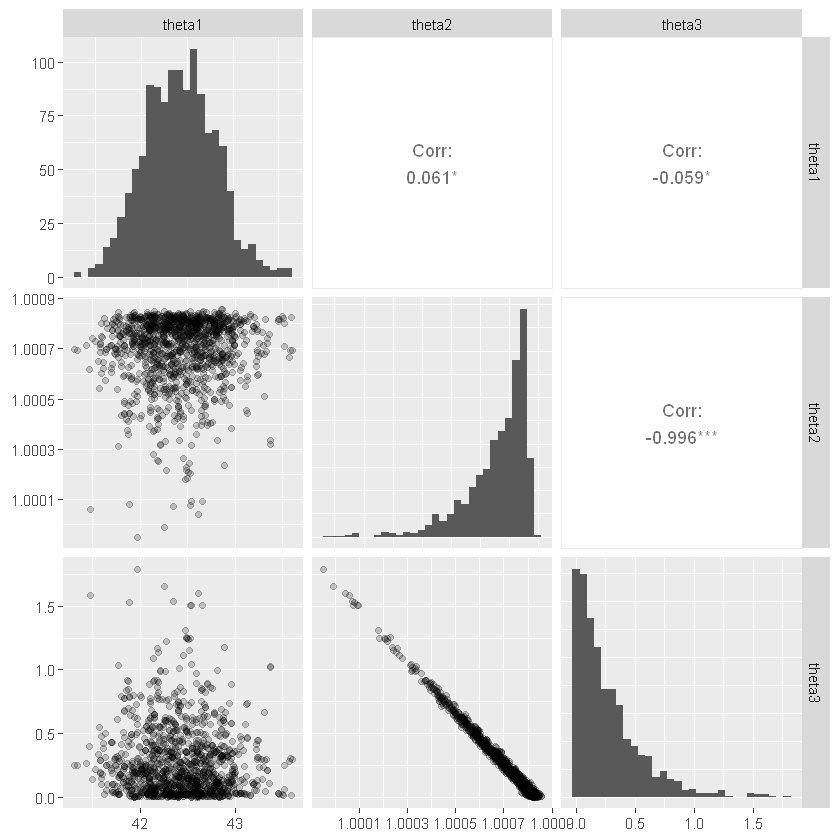
\includegraphics[width=0.9\textwidth, height=0.55\textheight]{pairplot.png}
  \caption{Histogram of $\theta_i$ and the pairwise scatterplot of $\theta_i, \theta_j$}
  \label{fig:pairplot}
\end{figure}
However, when we examine the plot of regression for the true data (See Figure \ref{fig:regrssion}), we see that the regression curve is not a very good fit of the data. This is probably due to the misspecification of the model. From EDA, it can be observed that the amplitude of the cycle of data should be increasing with time, while in our model, the amplitude is a fixed $\theta_1$.
\begin{figure}[!ht]
  \centering
  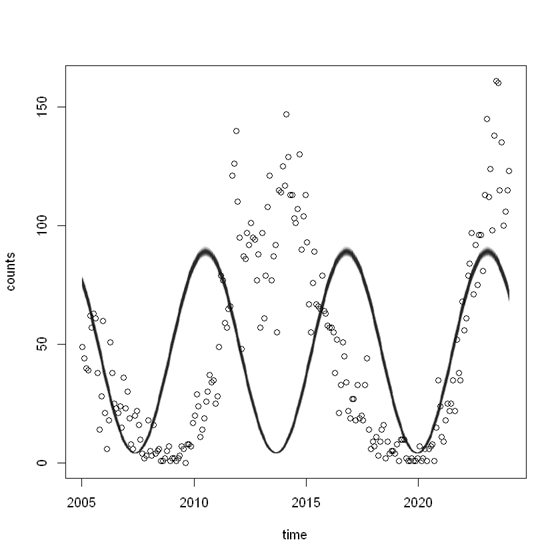
\includegraphics[width=\textwidth, height=0.6\textheight]{regression.png}
  \caption{Regreesion plot}
  \label{fig:regrssion}
\end{figure}






\qsol{A simple MCMC algorithm}
\begin{enumerate}
\item 
\begin{lstlisting}[language=R]
  # prior: Beta(alpha, beta)
  alpha = 1
  beta = 2 
  
  # observations: binomial draws
  n_successes = 3 
  n_trials = 3
  
  gamma_beta_binomial = function(p) {
      if (p < 0 || p > 1) {
          return(0.0)
      }
      dbeta(p, alpha, beta) * dbinom(x = n_successes, size = n_trials, prob = p)
  }
  
  simple_mh = function(gam, initial_point, n_iters) {
    samples = numeric(n_iters) 
    dim = length(initial_point)
    curr = initial_point
    # gamma(x) == 0 ==> ratio undefined; while gamma(x') = 0 only makes repeated samples
    # exception handling
    if (gam(curr) == 0) {
      print("Invalid initial point!")
      return(samples)
    }
    for (i in 1:n_iters) {
      proposed = rnorm(dim, curr, 1)
      accept_prob = min(1, gam(proposed)/gam(curr))
      u = runif(1, 0, 1)
      if (u <= accept_prob) {
        samples[i] = proposed
        curr = proposed
      }
      else {
        samples[i] = curr
      }
    }
    return(samples)
  }
  \end{lstlisting}
  \begin{lstlisting}[language=R]
    set.seed(2025)
    samples = simple_mh(gamma_beta_binomial, 0.5, 1500)
    mean(samples) # 0.66855402470144
    median(samples) # 0.678378290695954
  \end{lstlisting}


\item 
We wish to compute the theoreatical $\E(p | Y = 3)$, so given $p \sim \Beta(1,2)$ and $Y|p \sim \Bin(3, p)$, we have: $\gamma(p) = (1-p)p^3$, so it means the posterior density $\pi(p) \propto p^3(1-p)$, hence $p|Y=3 \sim \Beta(4,2)$, so $\E(p | Y=3) = \frac{4}{4+2} = \frac23$.


\end{enumerate}




% Optional: Feedback on assignment
% \qsol{Feedback on assignment}

 
\end{document}

